% Conteudo do capitulo
%1- Razoes fisicas para se ter o ATLAS UPGRADE 
%2- Porque a melhor escolha para o upgrade e o LGAD
%3- Importacia cientifica do LGAD
%4- Introducao ao LGAD
%5- Proposta do projeto
%6- Alguns detalhes sobre o escopo do projeto
%7- Importancia para o grupo 
\chapter{Introdução}

Na última década, o experimento ATLAS no LHC foi extremamente importante, fornecendo informações sobre as propriedades do bóson de Higgs e contribuindo para valiosas descobertas no campo da física nuclear e de partículas \cite{atlas_rev}. Tendo em mente esse grande legado para a física, atualmente o experimento ATLAS, e o LHC, estão se preparando para iniciar uma nova etapa na pesquisa científica com o objetivo de atingir níveis de sensibilidade e precisão nas medidas que vão muito além dos níveis atuais \cite{tdr}, e cobrir áreas de pesquisa importantes, ainda não exploradas, no contexto do modelo padrão (SM), propriedades do bóson de Higgs e a busca por assinaturas físicas que estão além do modelo padrão.

Diversas medidas feitas para estudar o modelo padrão, bem como as propriedades do bóson de Higgs, são limitadas por incertezas sistemáticas presentes nos dados. Dessa forma é importante que os detectores sejam capazes de diminuir essas incertezas relacionadas com a reconstrução dos objetos físicos - e.g. jatos de partículas - e com a modelagem do fundo presente nos eventos reconstruídos. Com esse objetivo, melhorias na razão sinal-fundo e o aumento da estatística dos dados são necessárias para aumentar a precisão dos observáveis físicos. %Neste contexto, o \textit{High Granularity Timing Detector} (HGTD) será um detector importante para a melhoria na reconstrução de objetos físicos na região frontal do experimento ATLAS, permitindo alcançar níveis de precisão similares aos obtidos para a região de pseudo-rapidez central. Isso permitira reduzir substancialmente o erro sistemático nesse espaço de fase, e explorar com grande precisão os fenômenos físicos nessa região.

% 1 - Razoes físicas para se ter o ATLAS UPGRADE 
Neste contexto, para o experimento ATLAS, um dos desafios experimentais é reconstruir a trajetória das partículas na região de rapidez dianteira, produzidas na interação inicial, de modo a associá-las corretamente com o vértice onde foram originadas, em um regime de altas taxas de colisão. Para solucionar esse desafio, um novo sistema de detecção frontal, denominado HGTD ({\it High Granularity Timing Detector}), está sendo desenvolvido - com base nos sensores LGAD ({\it Low Gain Avalanche Detector}) - para fornecer uma medida precisa de tempo, com o objetivo de diminuir as incertezas experimentais na reconstrução dos eventos, e fornecer uma precisão na medida similar ao obtido para a região de pseudo-rapidez central \cite{tdr}.

Como ilustra a Fig. \ref{hgtd}, o HGTD foi desenhado para ser instalado na região dianteira do experimento, simetricamente separados a uma distancia de $3.5m$ do ponto de interação do feixe, região a qual está localizada após o volume do ATLAS {\it Inner Tracker} (ITk) \cite{tdr}.

\thispagestyle{plain}
%Com o aumento significativo da precisão na medida de partículas frontais, através do uso do HGTD, será possível medir com precisão a luminosidade do feixe, a qual é uma medida crítica para a determinação da seção de choque da produção de partículas em diversas analises físicas, além de  permitir a reconstrução de jatos de partículas com grande precisão.
O HGTD também será capaz de medir a luminosidade instantânea a cada cruzamento de feixe, uma medida crítica no cálculo de seção de choque de processos físicos. A melhoria na capacidade de reconstrução de jatos - que será obtida com o HGTD - aumentará a sensibilidade do experimento, permitindo explorar observáveis antes não explorados devido aos limites experimentais \cite{tdr}.

\thispagestyle{plain}
\begin{figure} 
    \centering
    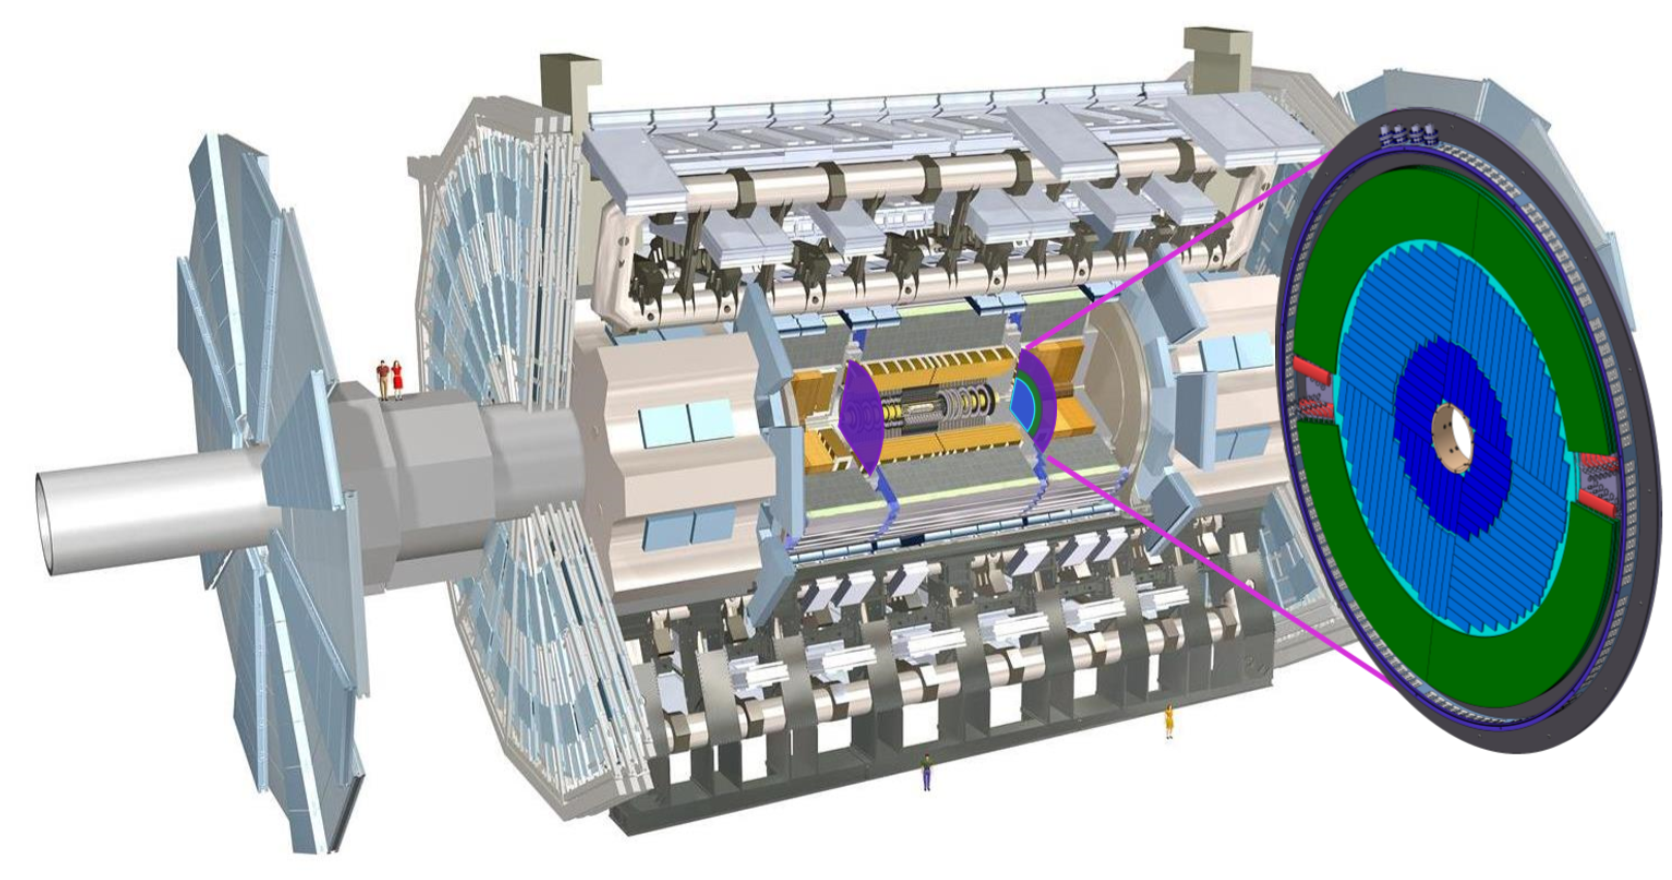
\includegraphics[width=15.0cm]{assets/ATLAS_HGTD.png}
    \caption{ Figura mostrando em detalhes a posição onde o HGTD será instalado. A figura também mostra o experimento ATLAS e os seus vários sistemas.}
    \label{hgtd}
\end{figure}

% 5 - PROPOSTA DO PROJETO
Em vista disso, o propósito deste projeto é desenvolver técnicas e metodologias experimentais necessárias para a caracterização física de sensores semicondutores do tipo LGAD para o upgrade do experimento ATLAS no CERN, bem como participar na construção do primeiro protótipo do HGTD e sistemas associados.

\section{Sensores LGAD}

O sensor LGAD foi adotado como base tecnológica para a construção do HGTD por apresentar excelentes características com respeito ao compromisso entre ganho e resolução temporal \cite{tdr,JIN_LGAD,NIMA_LGAD,NIMA_LGAD_I,NIMA_LGAD_II,NIMA_LGAD_III}. Além da resposta rápida à incidência de radiação, esse tipo de sensor possui ganho intrínseco devido ao perfil de dopagem empregado no material semicondutor, o que torna possível amplificar o sinal produzido e dessa forma operá-lo em modo de avalanche de carga \cite{JIN_LGAD,NIMA_LGAD,NIMA_LGAD_I,NIMA_LGAD_II,NIMA_LGAD_III}. Essas características comprovam a importância dessa tecnologia para o desenvolvimento da próxima geração de sensores semicondutores para aplicações que requerem altas taxas de contagem e ganho moderado.
\thispagestyle{plain}

Como ilustra a Fig. \ref{lgad}, LGAD são sensores semicondutores planos com ganho intrínseco. O ganho do sensor é determinado pela quantidade de dopante implantado na matriz de silício formando a camada de multiplicação. Como mostra a Fig. \ref{lgad}, sua arquitetura é composta de uma camada de material semicondutor do tipo n sobre uma camada do tipo p, com a adição de uma camada altamente dopada do tipo p localizada entre a junção n-p, cuja função é criar um alto campo elétrico responsável por produzir a avalanche das cargas, amplificando o sinal elétrico. Dessa forma, quando uma partícula atravessa a região sensível do detector, elétrons e lacunas são criados produzindo uma corrente inicial. Os elétrons ao atingirem a região de amplificação produzem novos pares elétron lacuna sendo desse modo multiplicados em um processo de avalanche, produzindo uma corrente de 10 a 30 vezes maior do que a gerada pelas ionizações primárias \cite{JIN_LGAD,NIMA_LGAD_III}. 

\begin{figure}
    \centering
    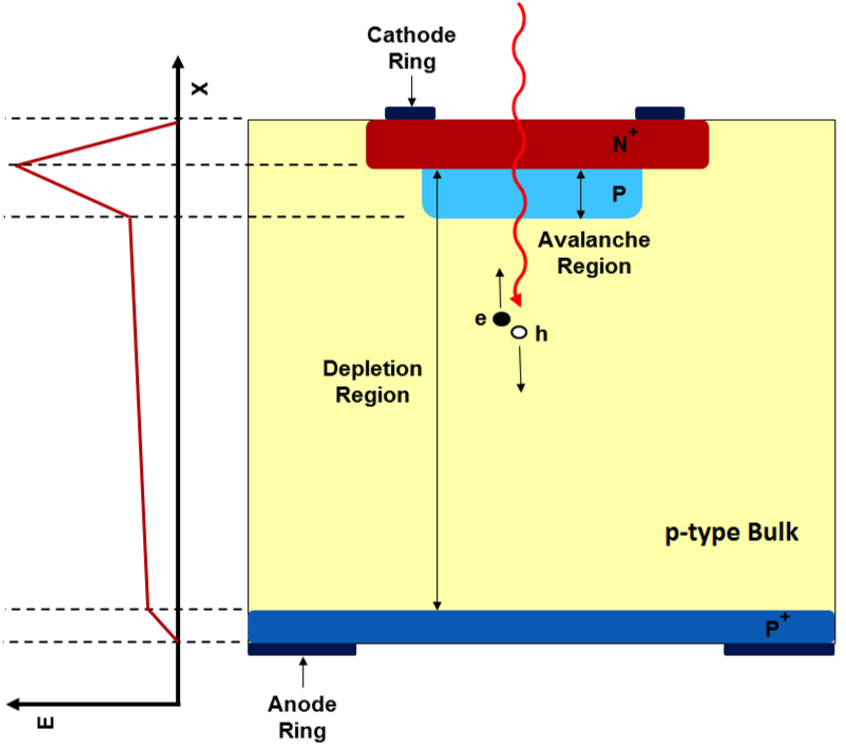
\includegraphics[width=7.0cm]{assets/lgad.png}
    \caption{Figura mostrando a estrutura esquemática de um sensor LGAD.}
    \label{lgad}
\end{figure}
\thispagestyle{plain}

\section{Protótipo do HGTD}

A Fig. \ref{hgtd}.a mostra o módulo híbrido do HGTD composto pelo sensor LGAD, dois ASICs - responsáveis pela aquisição do sinal - que juntamente com o LGAD formam o denominado \textit{bare module}, e as placas de circuito impresso flexível, compostas por duas partes, uma colada permanentemente no \textit{bare module} denominada \textit{Module Flex}, e a outra que se estende ao longo do detector, \textit{Flex Tail}. O sensor LGAD e os ASICs serão conectados através de uma solda de ligação. Todas as conexões entre o ASIC e a eletrônica de aquisição de dados serão feitas através do circuito impresso flexível, \textit{Module Flex}, onde o ASIC é conectado ao circuito através de fios soldados entre ambos.    

A Fig. \ref{hgtd}.b mostra o detalhe três módulos colados precisamente sobre a placa de refrigeração e posicionados ao longo da direção z do HGTD. Na figura é possível visualizar os cabos flexíveis, \textit{Flex Tail}, responsáveis por transmitir os sinais do ASIC, e fornecer os serviços de alimentação de baixa tensão, e alta tensão para os sensores. 

Como mostra a Fig. \ref{hgtd}.c, o protótipo do HGTD será composto de uma placa de refrigeração, onde dez módulos serão precisamente colados. A eletrônica de aquisição e leitura dos dados será conectada através dos cabos flexíveis e protótipos das fontes de alimentação de alta e baixa tensão do sistema serão utilizadas. Por fim, serão efetuados testes de funcionamento com a detecção de raios cósmicos e raios-X.    

\begin{figure}
    \centering
    \subfloat[a]{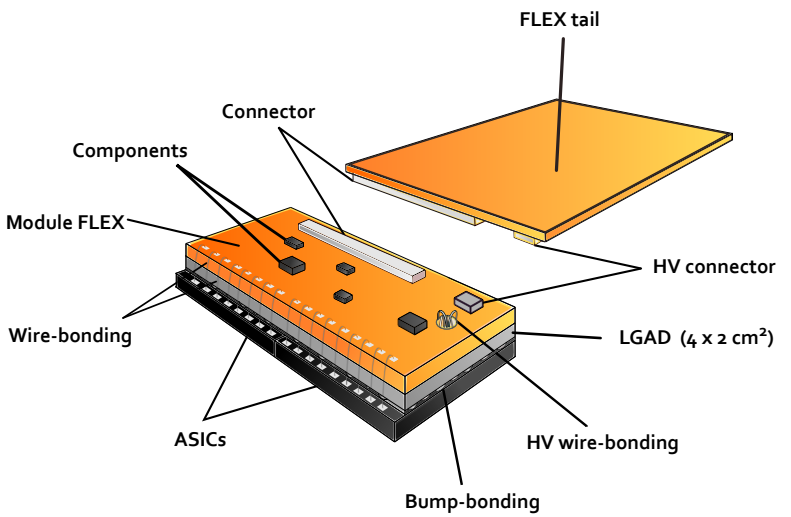
\includegraphics[width=7.0cm]{assets/HGTD_module.png}}
    \subfloat[b]{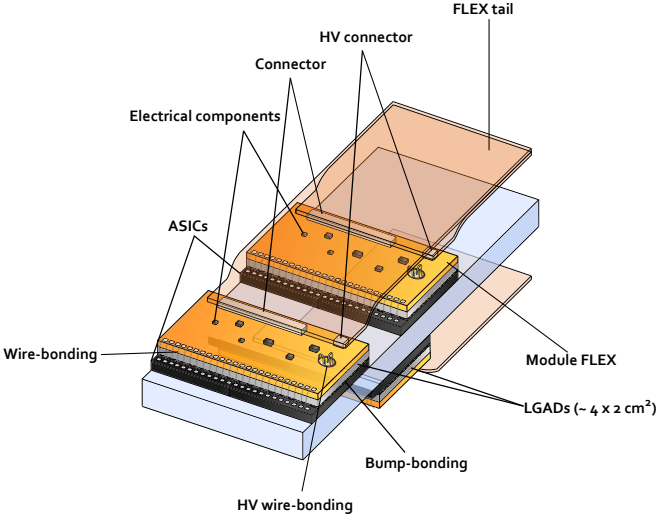
\includegraphics[width=7.0cm]{assets/HGTD_Prototype.png}}
    \subfloat[c]{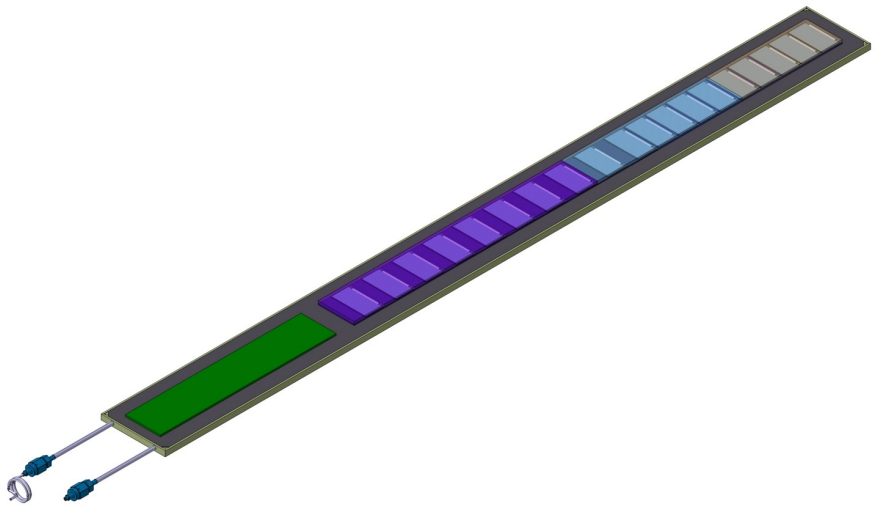
\includegraphics[width=7.0cm]{assets/HGTD_Mec_Module.png}}
    \label{hgtd}
    \caption{Figura mostrando os componentes do HGTD. [a] Módulo híbrido do HGTD. [b] Três módulos colados na placa de refrigeração. [c] Estrutura mecânica da placa de refrigeração.}
\end{figure}
\thispagestyle{plain}
\renewcommand{\cleardoublepage}{}
\renewcommand{\clearpage}{}